% ----- Consignes exo 1 ----- %
%
% \section*{TD1 --- First sheet title}\label{sec:TD1}
% \addcontentsline{toc}{section}{\nameref{sec:TD1}}

\iftoggle{showquestions}{
    \begin{td-exo}[Antigone des asso]\,\\ % 1
        Un groupe de personnes est tel que:
        \begin{enumerate}
            \item Chaque personne est membre d'exactement deux associations,
            \item chaque association comprend exactement trois membres,
            \item deux associations ont toujours exactement un membre en commun.
        \end{enumerate}
        Combien y a-t-il de personnes? D'associations?
    \end{td-exo}
}{}

% ----- Solutions exo 1 ----- %
\begin{td-sol}[]\,\\ %
    Il y a exactement 6 personnes et 4 associations avec l'arrangement qui suit:

    \vspace{0.5cm}
    \ffigbox[\FBwidth]{%
\label{Fig:td1ex1c1}
}{
    \fbox{
        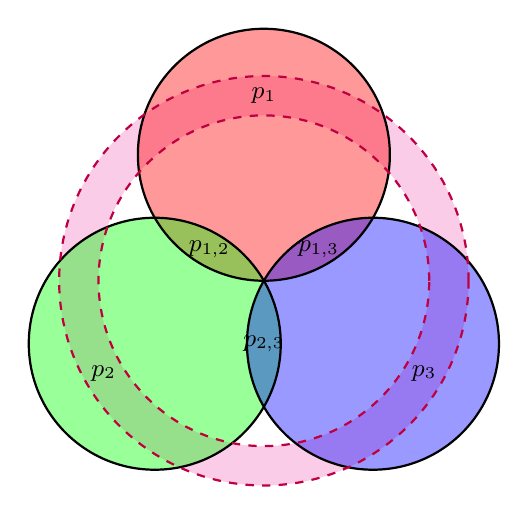
\begin{tikzpicture}[scale=1, every node/.style={circle, draw, fill=blue!20, inner sep=1pt, font=\scriptsize, minimum size=4mm}]
            % centers of the three circles
            \coordinate (A) at (90:1.6cm);
            \coordinate (B) at (210:1.6cm);
            \coordinate (C) at (330:1.6cm);
            \def\r{1.6cm} % radius (adjust as desired)
            
            % Add the circular band/strip
            \def\bandInnerRadius{2.1cm}
            \def\bandOuterRadius{2.6cm}

            % Draw the band with some transparency
            \fill[magenta, fill opacity=0.2] (0,0) circle (\bandOuterRadius);
            \fill[white] (0,0) circle (\bandInnerRadius);

            % draw filled circles with transparency
            \fill[red,   fill opacity=0.4]  (A) circle (\r);
            \fill[green, fill opacity=0.4]  (B) circle (\r);
            \fill[blue,  fill opacity=0.4]  (C) circle (\r);

            % remove (mask out) the triple-intersection area
            \begin{scope}
                \clip (A) circle (\r);
                \clip (B) circle (\r);
                \clip (C) circle (\r);
                % filling a large rectangle inside the triple-clip erases that area
                \fill[white] (-3,-3) rectangle (3,3);
            \end{scope}

            % circle outlines
            \draw[line width=0.8pt] (A) circle (\r);
            \draw[line width=0.8pt] (B) circle (\r);
            \draw[line width=0.8pt] (C) circle (\r);
            
            % Optional: Add outline for the band
            \draw[line width=0.8pt, purple, dashed] (0,0) circle (\bandInnerRadius);
            \draw[line width=0.8pt, purple, dashed] (0,0) circle (\bandOuterRadius);

            % Updated labels - moved to intersections between strip and circles
            \node[circle, draw=none, fill=none, font=\small] at (90:2.35cm) {\(p_1\)}; % Top circle
            \node[circle, draw=none, fill=none, font=\small] at (210:2.35cm) {\(p_2\)}; % Bottom left circle
            \node[circle, draw=none, fill=none, font=\small] at (330:2.35cm) {\(p_3\)}; % Bottom right circle

            % Labels for pairwise intersections (unchanged)
            \node[circle, draw=none, fill=none, font=\small] at (30:0.8cm) {\(p_{1,3}\)}; % A∩C
            \node[circle, draw=none, fill=none, font=\small] at (150:0.8cm) {\(p_{1,2}\)}; % A∩B
            \node[circle, draw=none, fill=none, font=\small] at (270:0.8cm) {\(p_{2,3}\)}; % B∩C
        \end{tikzpicture}
    }
}

    On peut bien vérifier qu'avec les associations
    \begin{itemize}
        \item \(\color{red}A = \{p_1, p_{1,2}, p_{1,3}\}\),
        \item \(\color{green}B = \{p_2, p_{1,2}, p_{2,3}\}\)
        \item \(\color{blue}C = \{p_3, p_{1,3}, p_{2,3}\}\)
        \item \(\color{magenta}D = \{p_1, p_2, p_3\}\)
    \end{itemize}
    on respecte bien les trois contraintes:
    \begin{enumerate}
        \item Chaque personne est membre d'exactement deux associations:
        \begin{itemize}
            \item \(p_1\) est dans \(A\) et \(D\),
            \item \(p_2\) est dans \(B\) et \(D\),
            \item \(p_3\) est dans \(C\) et \(D\),
            \item \(p_{1,2}\) est dans \(A\) et \(B\),
            \item \(p_{1,3}\) est dans \(A\) et \(C\),
            \item \(p_{2,3}\) est dans \(B\) et \(C\).
        \end{itemize}
        \item Chaque association comprend exactement trois membres: 
        \begin{equation*}
            |A| = |B| = |C| = |D| = 3
        \end{equation*}
        \item Deux associations ont toujours exactement un membre en commun:
        \begin{itemize}
            \item \(A\cap B = \{p_{1,2}\}\),
            \item \(A\cap C = \{p_{1,3}\}\),
            \item \(A\cap D = \{p_1\}\),
            \item \(B\cap C = \{p_{2,3}\}\),
            \item \(B\cap D = \{p_2\}\),
            \item \(C\cap D = \{p_3\}\).
        \end{itemize}
    \end{enumerate}
\end{td-sol}


% ----- Consignes exo xx ----- %
\iftoggle{showquestions}{
    \begin{td-exo}[]

    \end{td-exo}
}{}

% ----- Solutions exo xx ----- %
\begin{td-sol}[]\ %
    % TODO: completer solution exercice xx
\end{td-sol}
